% You should title the file with a .tex extension (hw1.tex, for example)
\documentclass[11pt]{article}

\usepackage{bmpsize}
\usepackage[pdftex]{graphicx}
\usepackage{amsmath}
\usepackage{amssymb}
\usepackage{amsthm}
\usepackage{fancyhdr}
\usepackage[margin=2.5cm]{geometry}
\newcommand{\Ohm}{\Omega}
\newcommand{\inv}{^{-1}}
\renewcommand{\part}[1] {\vspace{.10in} {\bf (#1)}}


\pagestyle{fancyplain}


\begin{document}
\title{Digital Lab}
\author{David Galbraith}
\maketitle
%COMMENT: In Latex, using the maketitle function will perform all the formatting
%you had set up in the code below in a standard fashion

\normalsize
\begin{abstract}  %Abstract: \\

For this lab, we covered a wide range of topics relevant to digital
radio. I don't know what the hell they were yet though. %TODO: Figure
                                %out what the hell they were

\end{abstract}
%COMMENT: It is customary to use the abstract environment for the
%abstract, and to not include a pagebreak after the abstract prior to
%the introduction in a scientific paper


\lhead{\fancyplain{}{\textbf{Lab 2}}}      % Note the different brackets!
\rhead{\fancyplain{}{David Galbraith}}
\medskip                        % Skip a "medium" amount of space
                                % (latex determines medium is)
                                % Also try: \bigskip, \littleskip

\thispagestyle{plain}

\section{Introduction}
%COMMENT: Sections and subsections have their own format that will make
%the divisions in what you wrote more clear, and will number themselves,
%allowing you to focus more on content rather than order
The foremost, most fundamental piece of physics relevant to digital
signal sampling is the Nyquist criterion. A signal is a
continuously-varying quantity, but a computer can only read its value a
finite number of times. The Nyquist criterion states that in order to
get sample data that approximates the actual shape of the signal, one
must sample at at least twice the frequency of the signal. \\

Another piece of physics often relevant to digital radio is signal mixing. To mix signals, one uses a signal mixer. The mixer takes as input two signals and outputs their product in the time domain. This turns out to be their convolution in the frequency domain by the Convoolution Theorem. A mixer can be either Single Side Band (SSB) or Double Side Band (DSB). A Double Sideband mixer outputs a wave given by the product of its two input waves. By the equation $\cos{a}\cos{b} = 1/2 * (\cos{(a - b)} + \cos{(a + b)})$, this output is equivalent to the sum of two waves whose frequencies are equal to the sum and difference of the frequencies of the input waves. A Single Sideband Mixer takes the additional step of filtering out one of these terms, so the output frequency is just one of $a - b$ or $a + b$.
%TODO FIR FIlter, 5/8 bandpass

\section{Experiments, Observations, Analysis and Interpretation} 


%COMMENT: Using \label{value} and \ref{value} will allow you to refer to
%a specific figure without worrying about the order in which you have
%them in your document. While this obviously matters somewhat in terms
%of the logical flow of you paper, it's really helpful if you're moving
%things around as you write your paper. I did this for the first figure,
%but you can change the rest fairly easily. Additionally, \centering
%will put the figure in the middle of the page when you scale it down to
%a more reasonable size.

\subsection{The Nyquist Frequency}

The first thing we did in this lab was try to understand and visualize
the Nyquist criterion. To do this, we sampled a signal at frequencies
ranging from 0.1 times the Nyquist frequency to 3 times the Nyquist
frequency and compared how effectively they seemed to illustrate the
underlying sinusoid. First we sampled at less than the Nyquist frequency: the resulting graphs appear in Figure \ref{nyql}. Then, we sampled at the Nyquist frequency and triple the Nyquist frequency: the resulting graphs appear in Figure \ref{nyqg}.
As you can see, the samples at less than the Nyquist frequency are
periodic, but it is not easy to see that the underlying signal is a
sinusoid or determine its amplitude or frequency. At the Nyquist frequency, the
signal is clearly sinusoidal, and its amplitude and frequency can be
easily determined. Finally, at triple the Nyquist frequency, the picture
smooths out even further and looks almost like a continuous waveform. 
\begin{figure}
\centering
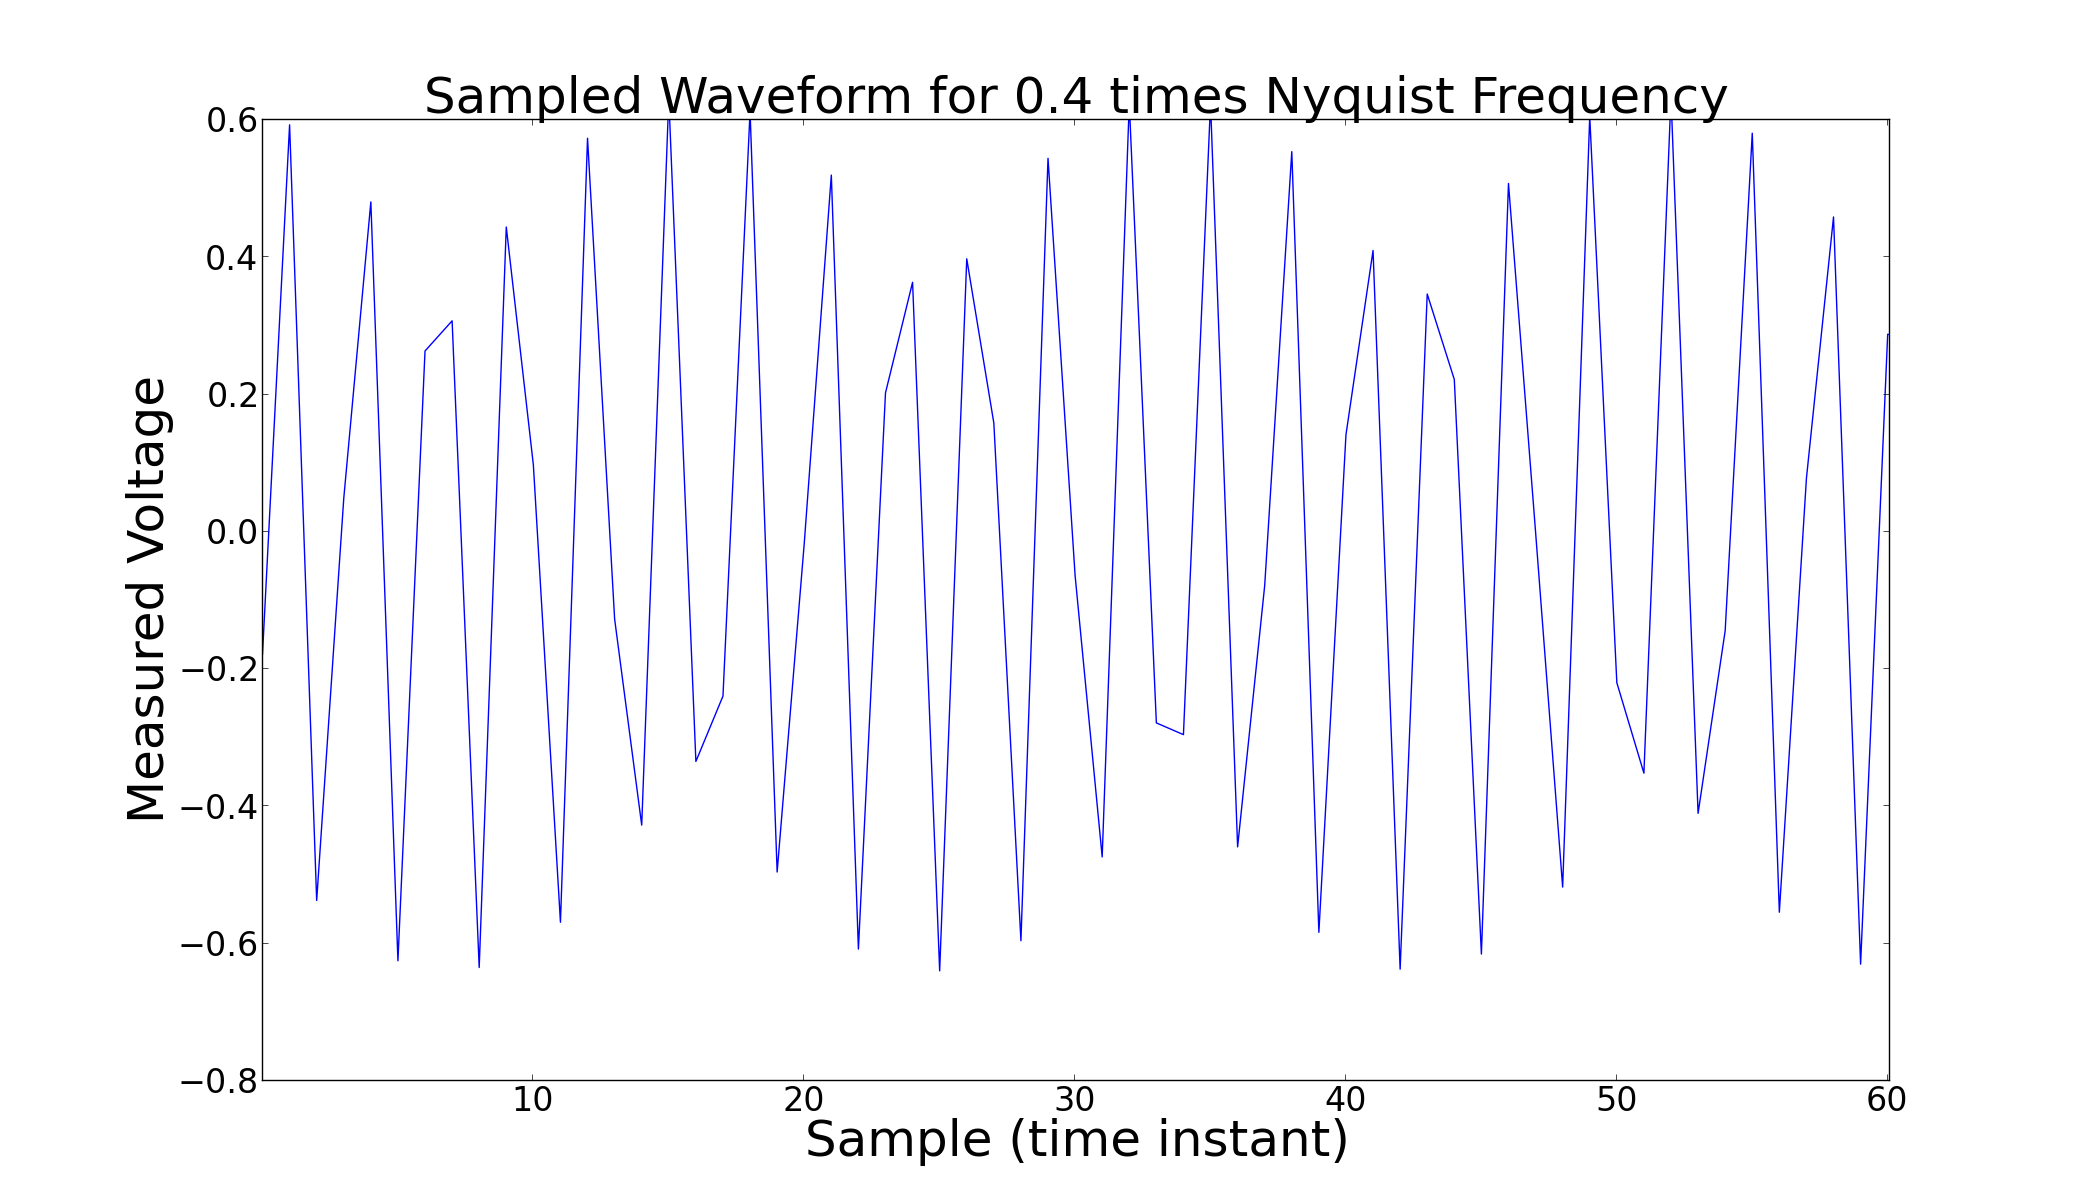
\includegraphics[scale=0.35]{pictures/pointfournyq}
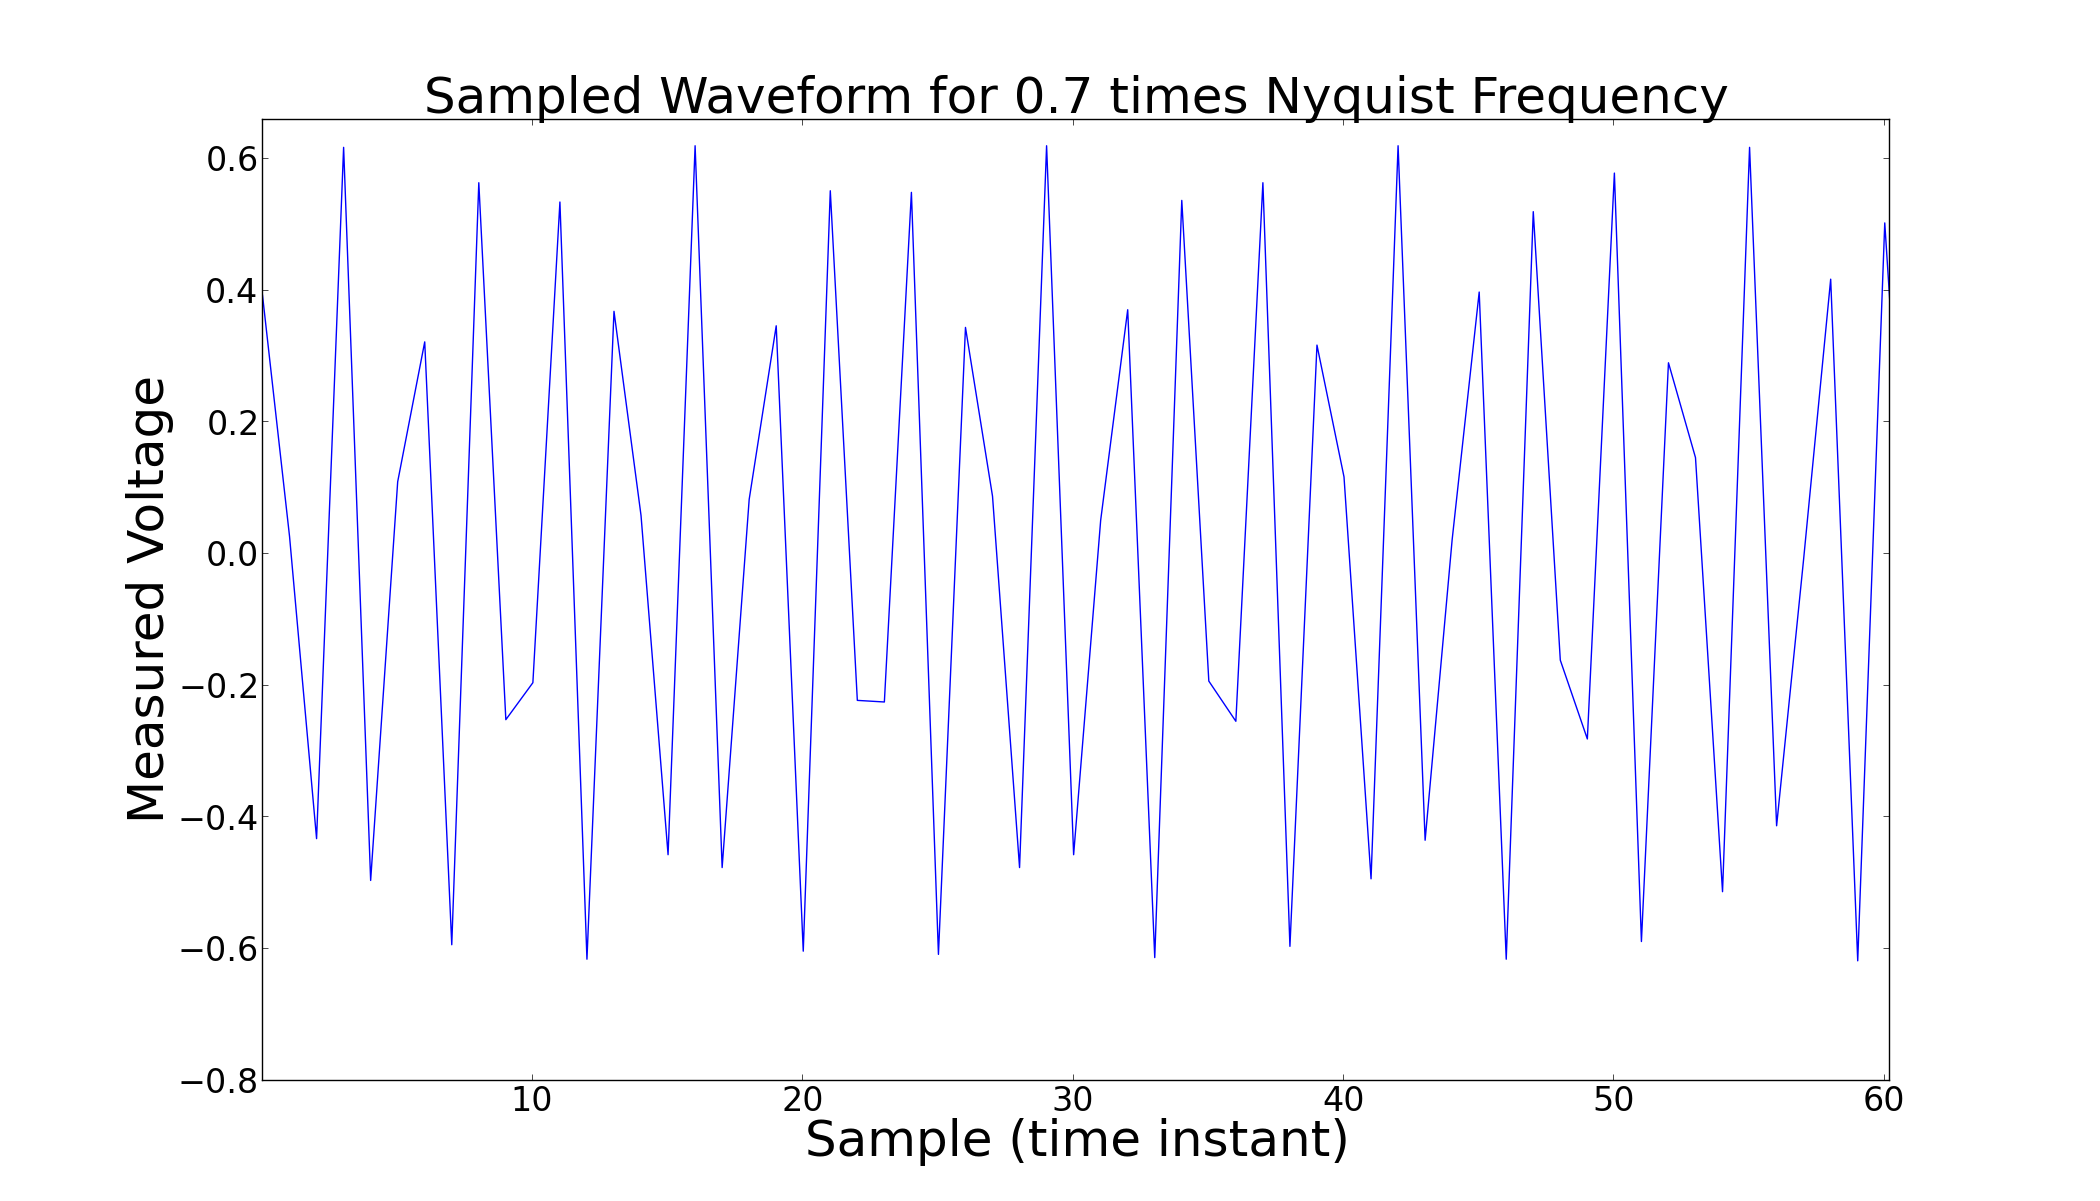
\includegraphics[scale=0.35]{pictures/pointsevennyq}
\caption{Sinusoidal signal sampled at 0.4 and 0.7
  times Nyquist frequency. \label{nyql}}
\end{figure}
\begin{figure}
\centering
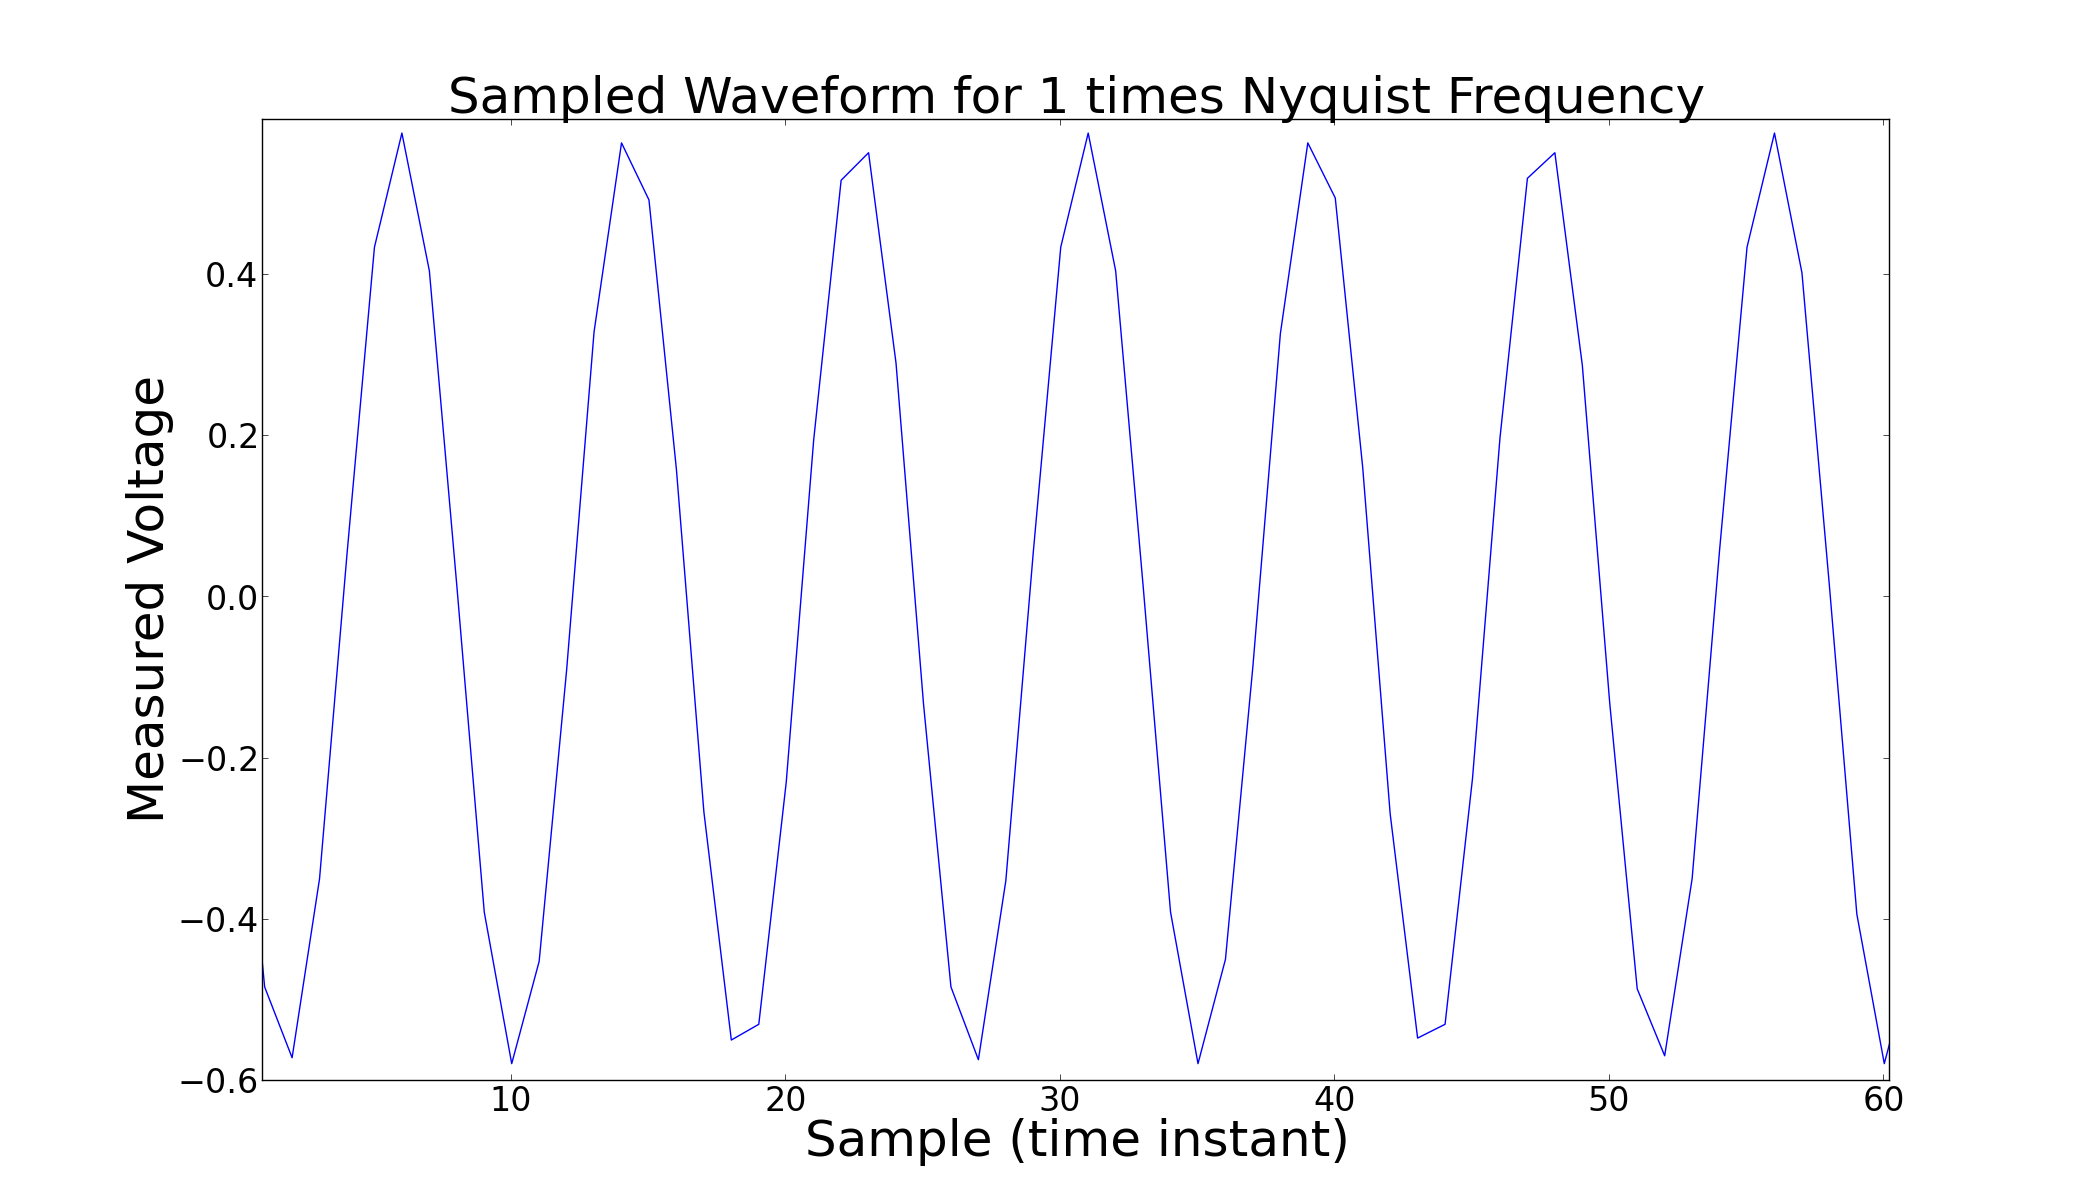
\includegraphics[scale=0.35]{pictures/onetimesnyq}
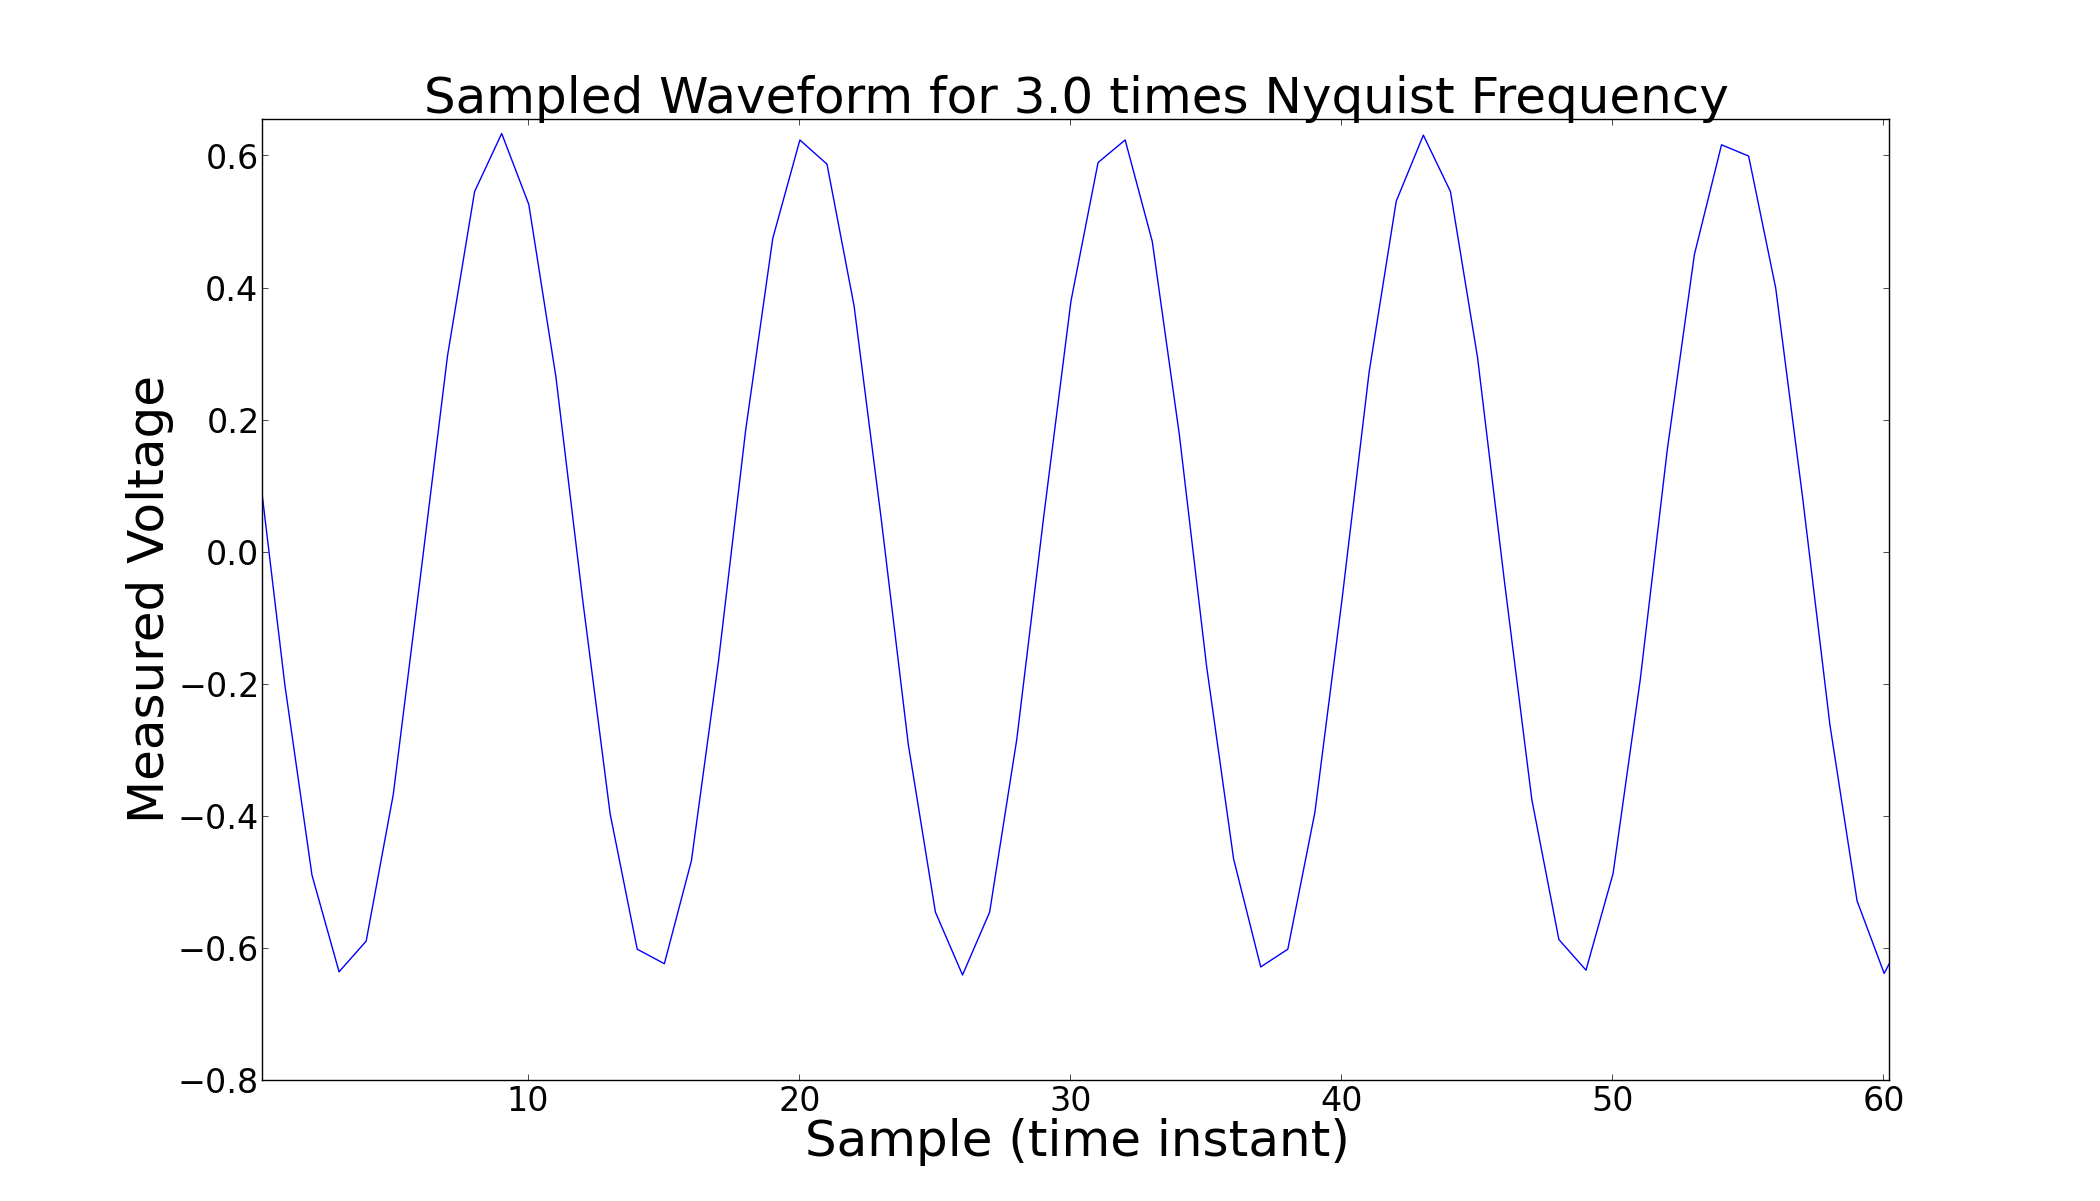
\includegraphics[scale=0.35]{pictures/triplenyq}
\caption{Sinusoidal signal sampled at 1 and 3
  times Nyquist frequency. \label{nyqg}}
\end{figure}
\subsection{Mixing}

In the second week of the lab, we used analog and digital mixers to combine waveforms generated by SRS generators and compared the outputs. First, we used an analog DSB to combine signals of 0.95 and 1.0 MHz as well as signals of 1.05 and 1.0 MHz. The waveform for the first case appears in Figure \ref{wavenine}. 

\begin{figure}
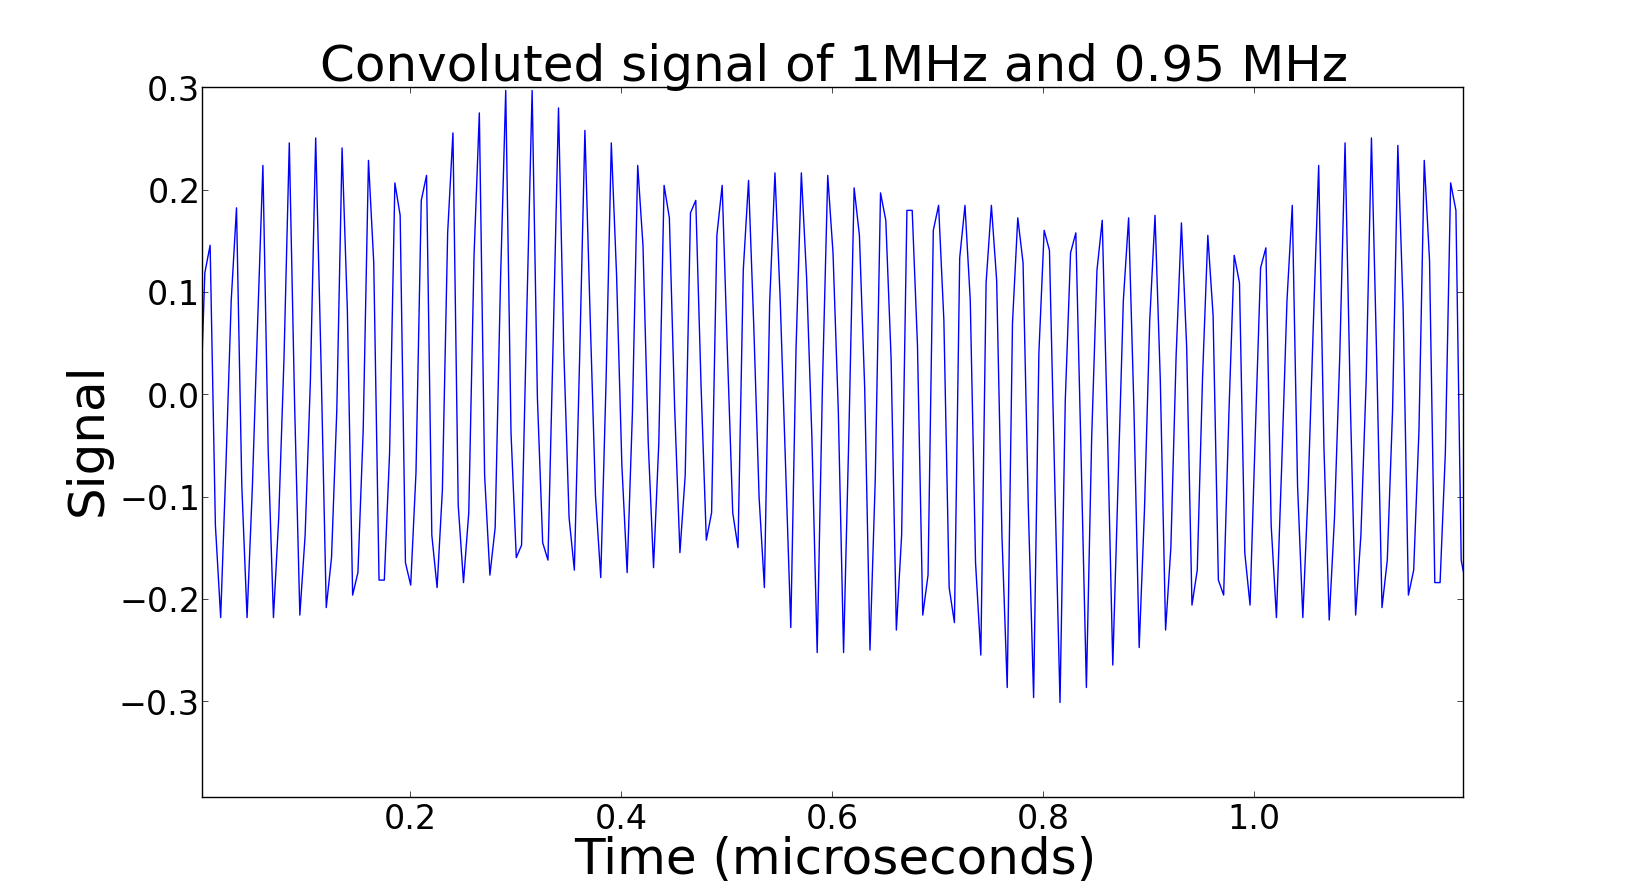
\includegraphics[scale=0.45]{pictures/signalninefive}
\caption{Convoluted signal of a 0.95 MHz wave and a 1.0 MHz wave \label{wavenine}}
\end{figure}

From the waveforms, we calculated the power spectrum using a Fourier transform: the results appear in Figure \ref{adsb}.

\begin{figure}
\centering
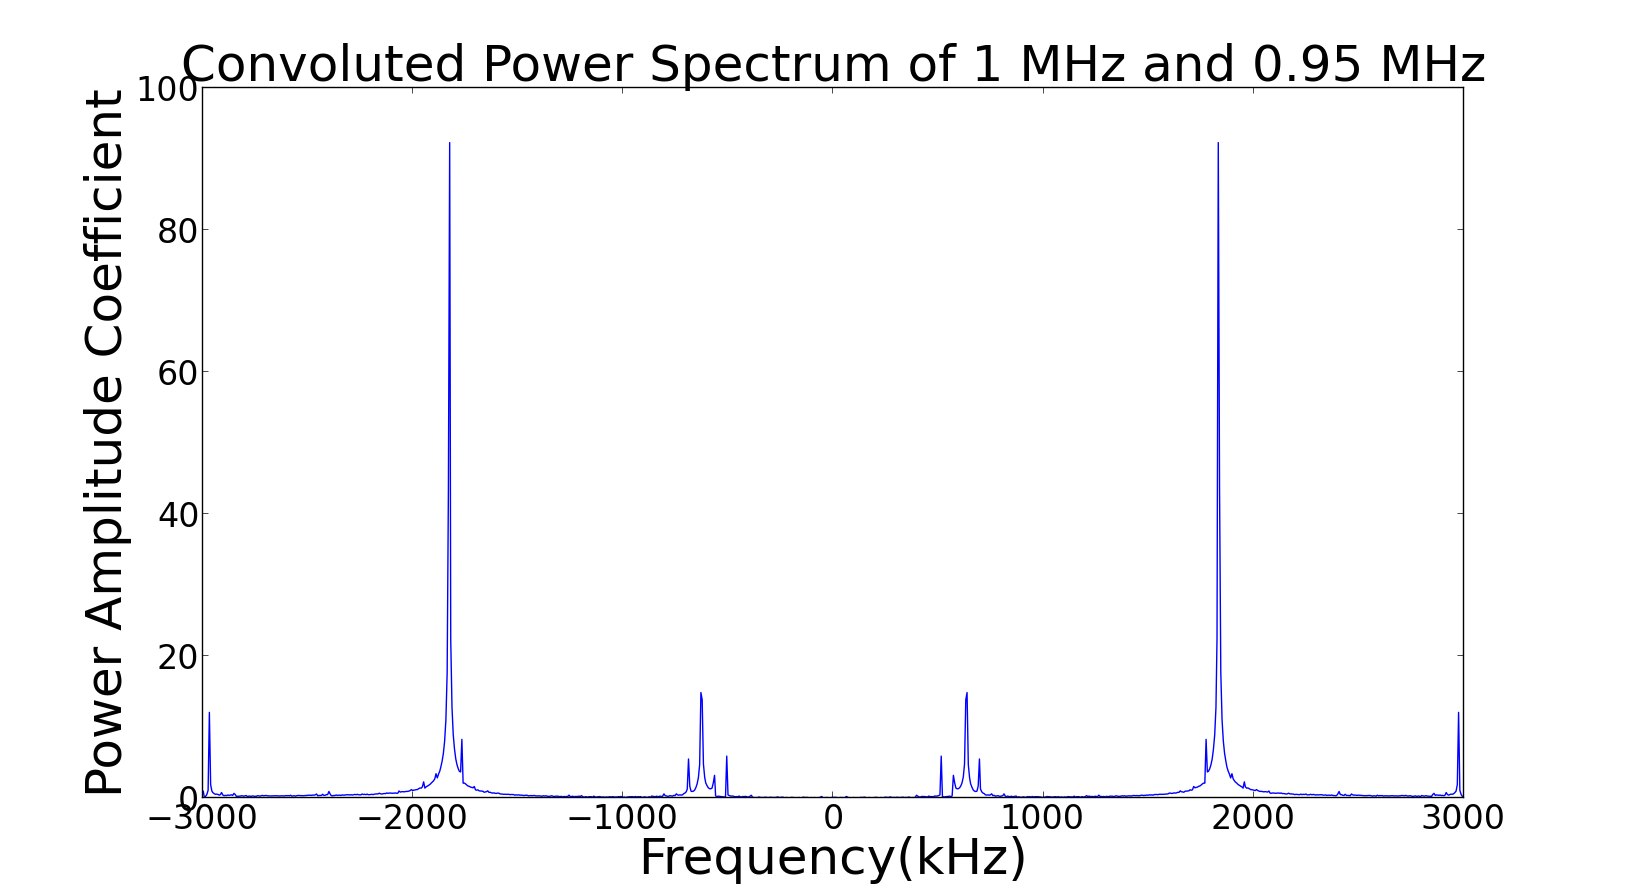
\includegraphics[scale=0.35]{pictures/opointninefive}
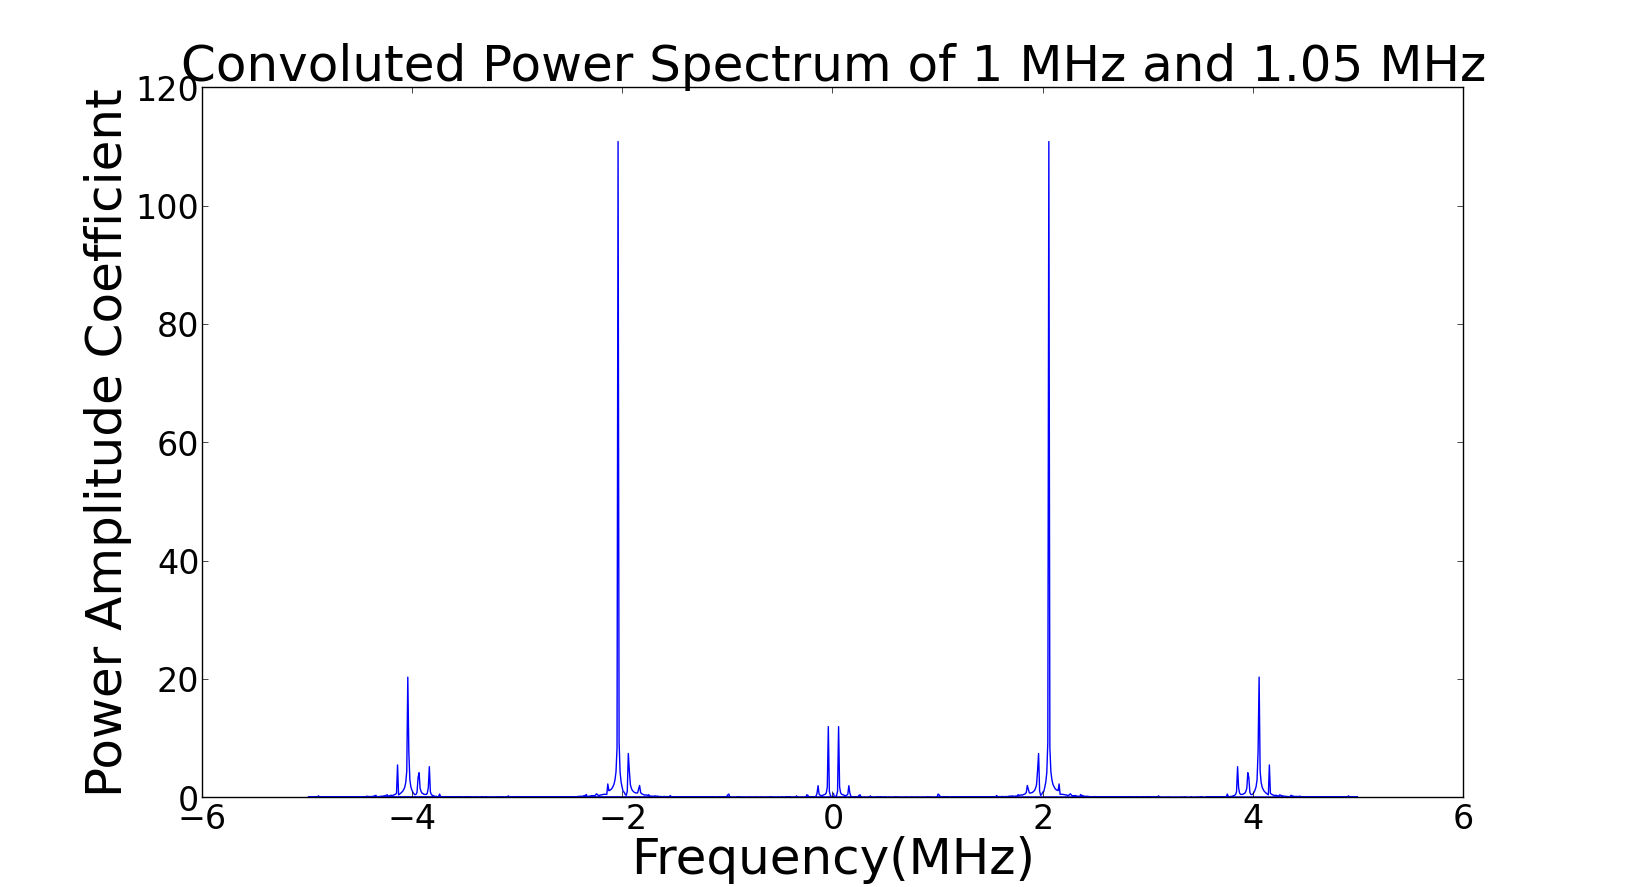
\includegraphics[scale=0.35]{pictures/onepointofive}
\caption{Analog DSB convolution power spectra of 0.95 MHz and 1.0 MHz (top), and 1.05 MHz and 1.0 MHz (bottom). \label{adsb}}
\end{figure}

 As you can see, the power amplitude coefficients strongly peak around 2 MHz, because that is roughly the sum of the frequencies we mixed. Looking closely, one can see that the highest peak of the mixture of 0.95 MHz and 1.0 MHz is at slightly less than 2 MHz, while the highest peak of the mixture of 1.05 and 1.0 MHz is slightly greater than 2 MHz, as expected. These peaks form the ``upper sideband'', the part of the spectrum centered at the sum of the input frequencies. In addition, you can see the ``lower sideband'' in the vicinity of 0 MHz, where the frequency is the difference of the input frequencies. Because we inadvertantly used too much power, the lower sideband is lower than the upper sideband, and some extra coefficients appear at $\pm 4$. Disregard these features. In addition, the whole distribution is reproduced on the negative side of the x-axis, because actual waveforms are complex exponentials, so the sine wave we mixed with is actually represented by $\sin{x} = 1/2 * i * (e^{-ix} - e^{ix})$, so we ended up convolving our 1.0 MHz local oscillator with waves of frequency 0.95 and -0.95 MHz  in the first case, and 1.05 and -1.05 MHz in the second case. Then, we filtered out the upper sideband of the convolved waveforms of Figure \ref{adsb} for the case of 0.95 MHz and found the IFFT of the lower sideband. The result appears in Figure \ref{ifft}. 

\begin{figure}
\centering
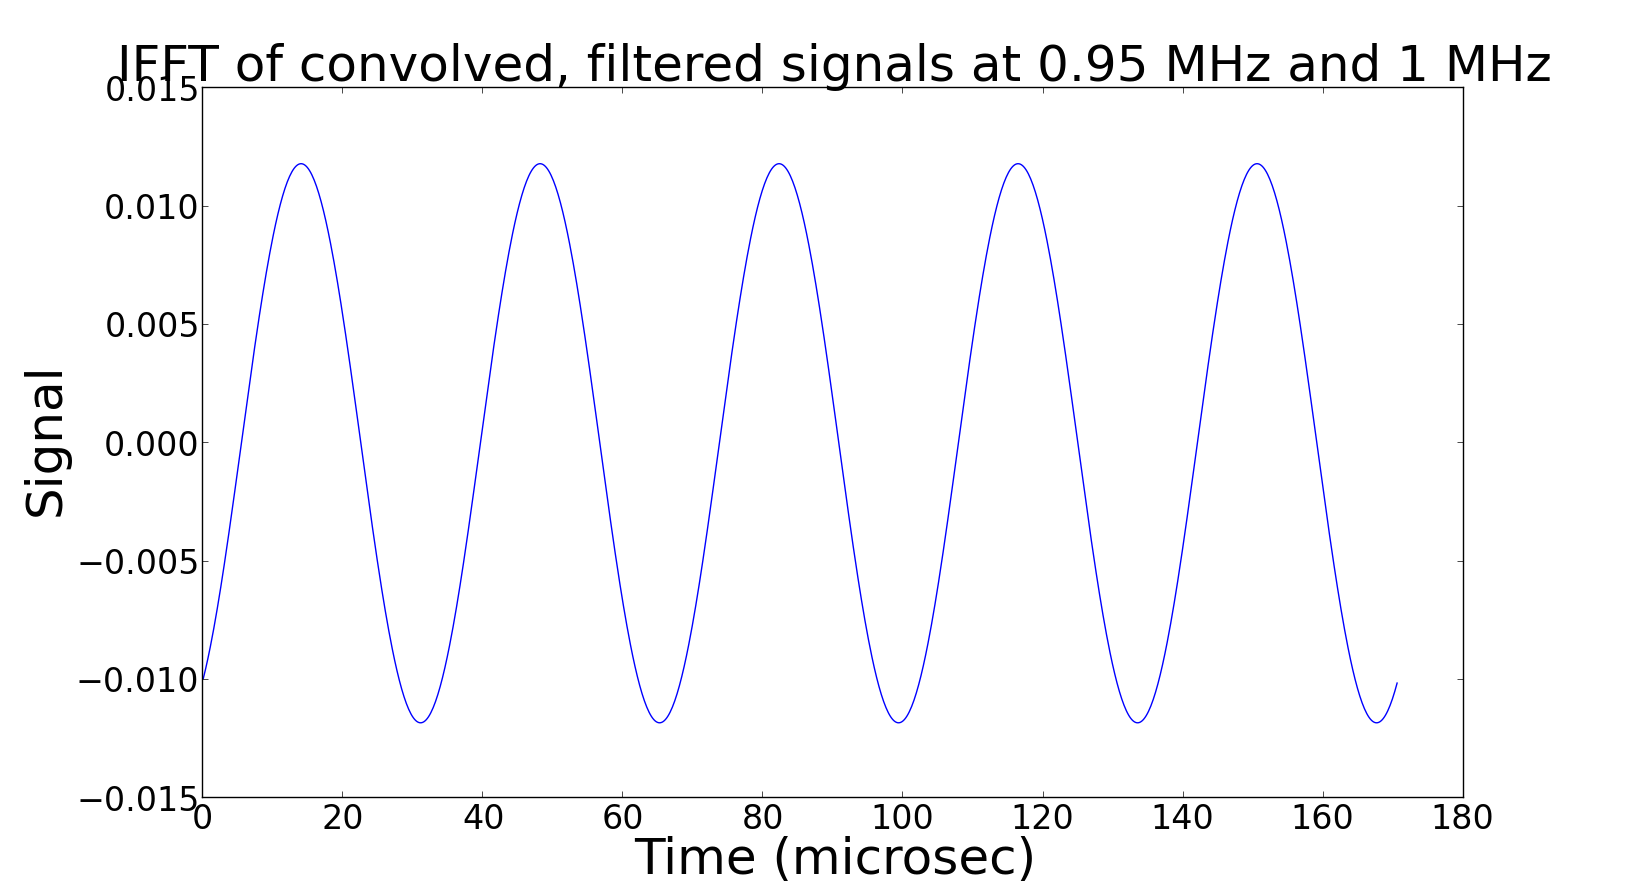
\includegraphics[scale=0.35]{pictures/ifft}
\caption{IFFT of lower sideband from convolved 0.95 and 1.0 MHz waves. \label{ifft}}
\end{figure}

The IFFT of the lower sideband is roughly a sinusoid with frequency 0.5 MHz. This makes sense because in the frequency domain it is sharply peaked about that frequency. The higher-order terms and noise errors contribute to small oscillations within the main 0.5 MHz oscillation. Finally, we made use of a digital mixer to explore DSB and SSB digital mixing. First, we used the digital DSB mixer to mix the same signals we mixed with the analog mixer above, and we compared the results. The digitally-mixed power spectrum appears in Figure \ref{digpow}.

\begin{figure}
\centering
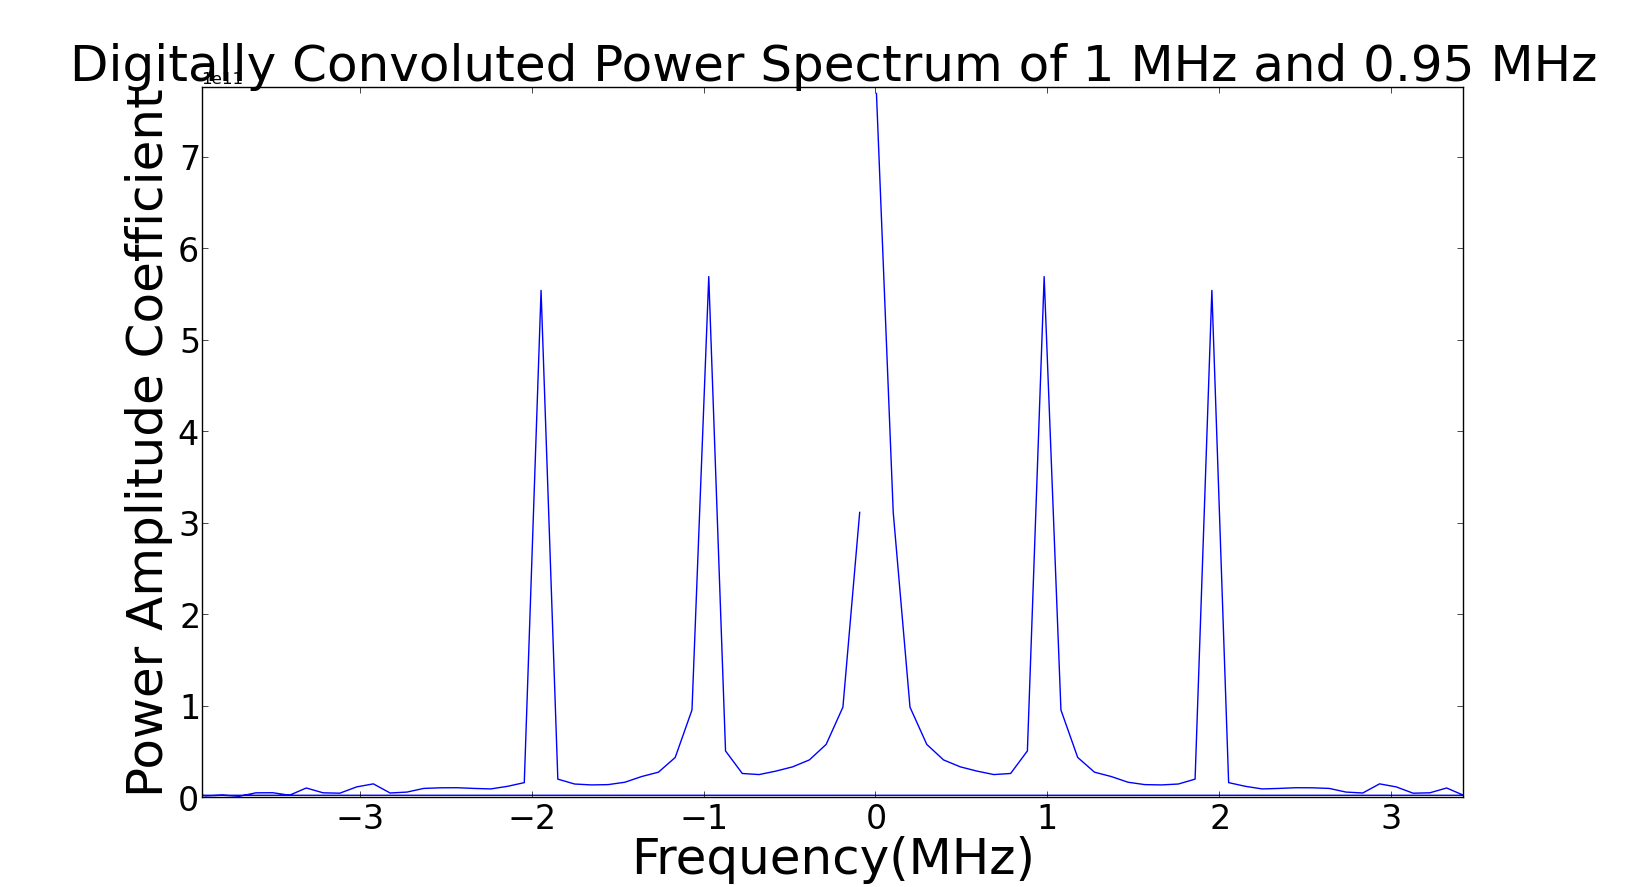
\includegraphics[scale=0.35]{pictures/digitaloninefive}
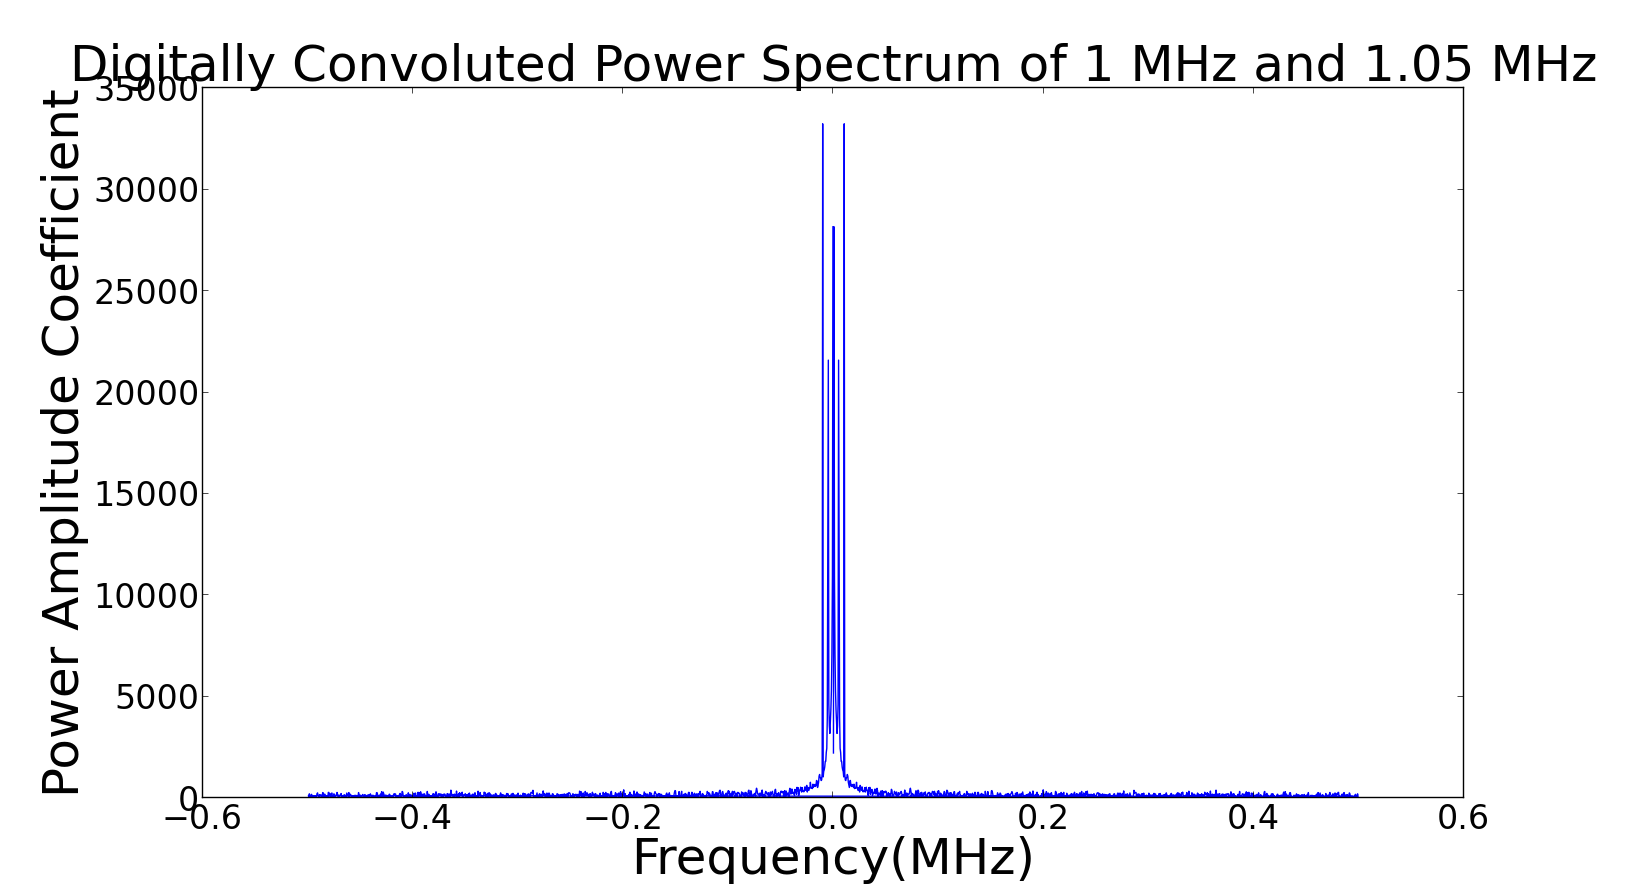
\includegraphics[scale=0.35]{pictures/digitaloneofive}
\caption{Power spectra for digitally mixed signals of 1 MHz and 0.95 MHz (top); 1 MHz and 1.05 MHz (bottom) \label{digpow}}
\end{figure}

Even though we mixed the same signals in the digital DSB mixer as in the analog DSB mixer, the graphs look different because of differences between digital and analog mixers. There are two differences relevant to this discussion. First, the digital mixer has a sort of implicit input in the form of a DC offset, which it mixes with the input signals. Second, the digital mixer has a resolution given by $\nu_s / N$, where $\nu_s$ is the sampling frequency and $N$ is the number of samples. Since the ROACH gives 2048 samples at 200 MHz, its resolution is roughly $200000000/2000 = 100$kHz. Signals whose frequencies are closer together than this resolution will be indistinguishable to the digital mixer. The digital graphs show five separate peaks. The center peak, at a frequency of 0, corresponds to the DC offset. In addition, since the difference frequencies $|1 - 1.05|$ and $|1 - 0.95|$ are equal to $50$kHz, which is less than the resolution, their power amplitudes are added to this center peak as well. The next peak to the right, around 1 MHz, is the sum of the input frequencies with the DC offset, whose frequency is zero. The resulting output signal has the same frequency as the input signal. Finally, around 2 MHz, there appears a spike corresponding to the output signal whose frequency is the sum of the two input frequencies. For the same complex-exponential reasons as in the analog case, the whole spectrum is reproduced on the negative side of 0.

Then, we used the SSB mixing functionality of our digital mixer to mix an input signal %TODO what input signal
with a local oscillator. %TODO the rest of 2.2

\section{FIR Filter}

In the last week of the lab, we designed an FIR filter to be a 5/8 bandpass. In the frequency domain, such a filter ideally has nonzero coefficients in the five frequencies closest to zero and zero coefficients elsewhere. We approximated these features with a sinc function, $\sin{x}/x$, which rapidly drops off except in the vicinity of 0. By computing the inverse FFT of the sinc function on eight points about zero, we found the time-domain coefficients that would Fourier transform into it, creating the 5/8 bandpass we desired. The resulting coefficients and their binary representations appear in Figure \ref{table}.
\begin{figure}
\centering
\begin{tabular}{c|c|c}
Register & Coefficient & Binary representation \\
-4 & 0.239389 & 0.00111101010010001 \\
-3 & 0.508846 & 0.10000010010000111\\
-2 & 0.759187 & 0.11000010010110100\\
-1 & 0.936155 & 0.11101111101001111\\
0 & 1.0 & 0.11111111111111111\\
1 & 0.936155 & 0.11101111101001111\\
2 & 0.759187 & 0.11000010010110100\\
3 & 0.508846 & 0.10000010010000111\\
\end{tabular}
\caption{Coefficients for our FIR filter. \label{table}}
\end{figure}

%TODO desired ideal filter response, actual calculated filter response

The actual effect of our FIR filter appears in Figure \ref{fir}. %TODO yaxis units, what are the different lines, get all the data together in one plot

\begin{figure}
\centering
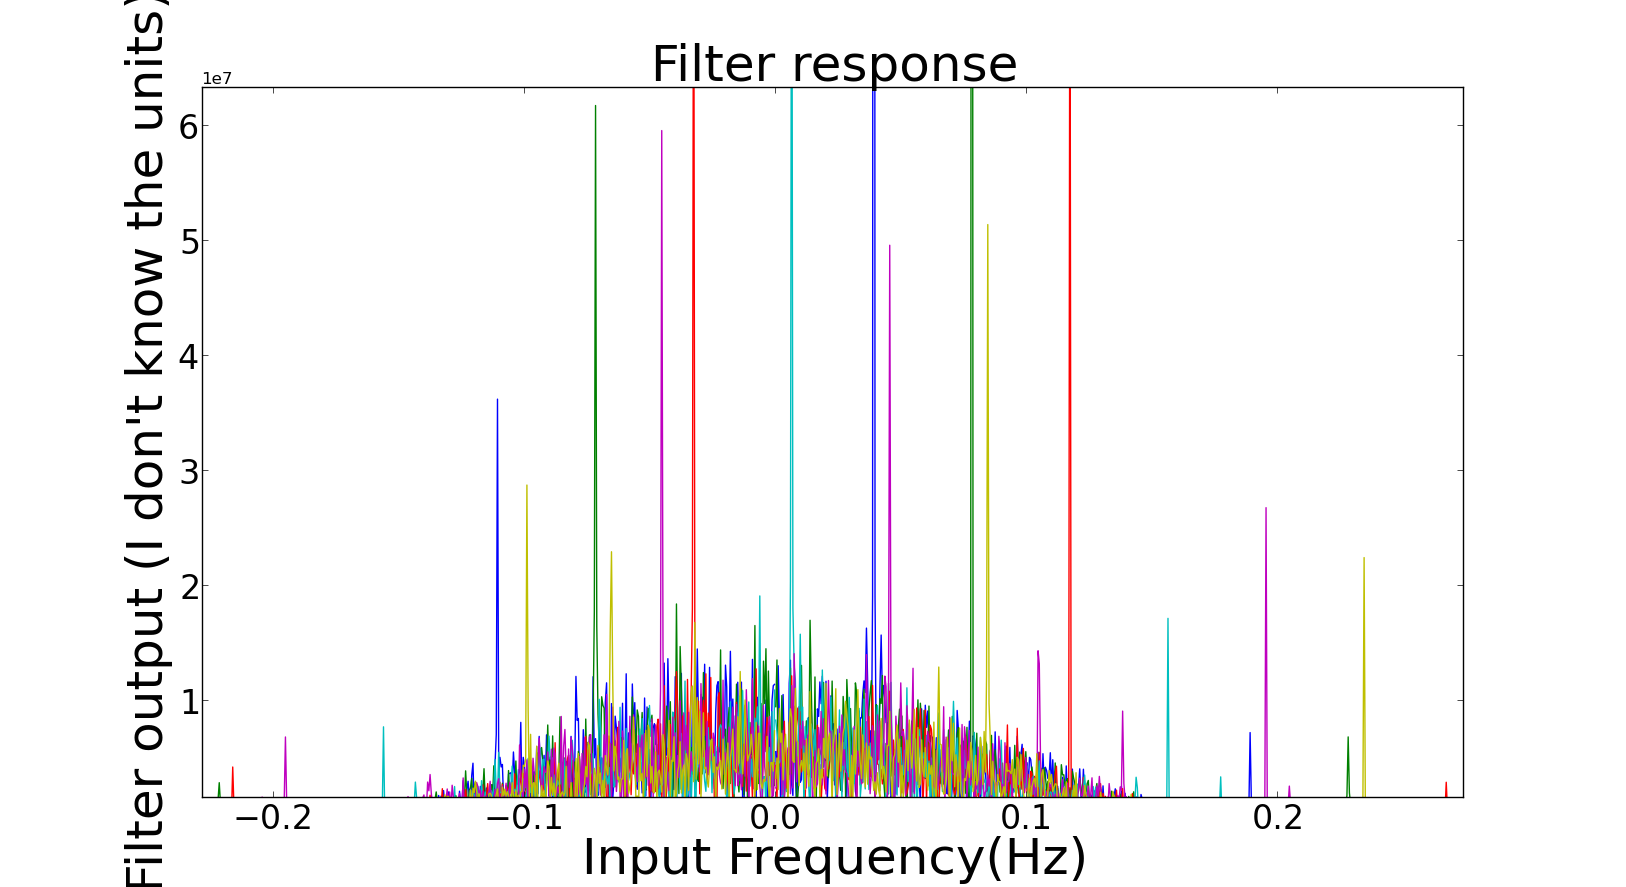
\includegraphics[scale=0.35]{pictures/fir}
\caption{Output of our FIR filter. \label{fir}}
\end{figure}

%COMMENT:By placing your figures in the flow of your text, you can
%increase the likelihood that they appear in reasonable places based on
%where you reference them. Combining figures (2 & 3 were combined) that
%are related or demonstrate two aspects of one thing can also allow you
%to use space in your paper more effectively.


%COMMENT: Captions should go below figures always.

This was a fun lab report and I love radios and stuff! %TODO the rest of the lab

%COMMENT: In a report you don't need to write out unit names, and it
%would actually be preferred you use things like $\mu$H versus mircoHenry

\end{document}
